\documentclass[twoside,11pt]{article}
\usepackage[top=1in, bottom=1in, left=1in, right=1in]{geometry}
\usepackage{amsmath,amsfonts,amsthm,fullpage}
\usepackage{algorithm}
\usepackage{algorithmic}
\usepackage{graphicx}
\usepackage{float}
\usepackage{url, apacite}
\usepackage{amsmath}
\usepackage{amssymb}

\graphicspath{ {../data/} }
\newcommand{\Fa}{$\mathbf{F_a}$}
\newcommand{\Fb}{$\mathbf{F_b}$}
\newcommand{\Fi}[1]{$\mathbf{F_{#1}}$}

\begin{document}

\title{CS6491-2015 P3: Worm}
\author{Xiong Ding, Subhajit Das}
\date{}
\maketitle
\begin{figure} [H]
    \centering
    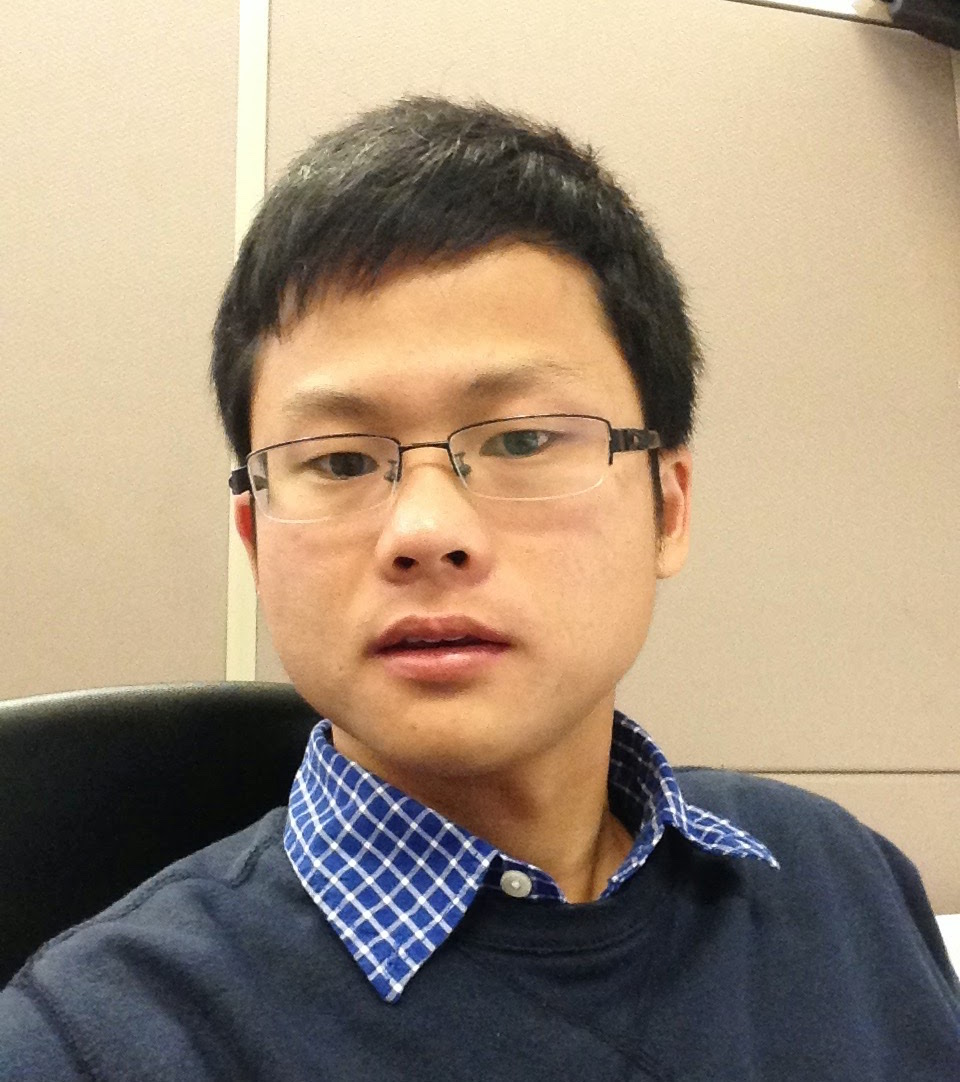
\includegraphics[width=0.9in]{selfie}
    
\includegraphics[width=1.0in]{das_PIC}
\end{figure}


%----------------------------------------------------------------------------------
\section{Objective}
Our objectives are the following:
 \begin{enumerate}
 \item Compute the median (average) curve between two input curves in a 3D space.
\item Animate a morph between two input curves 
\item Compute and display the inflation - “minimal” tube tangent to both input curves
 \end{enumerate}


\section{Definitions and input}
Given two curves $ A $ and $ B $ both sharing common start and end points in a 3D space. In order to make the morph between these curves,we will compute the medial curve $ C $ by computing the medial points $ M_1, M_2, M_3 ......M_N $.
Subsequently, we would make transverse curves in the form of a series of Arcs spaced at a combined distance of $D$ on each input curve, considering the two input curves can accommodate a sphere or ball of radius $ r $ in between them. Here, $D$ is the diameter of the biggest circle tangential to both curves $A$ and $B$.

\section{Approach}
\subsection{Definition of curves and the tangent vector}
Both curves $A$ and $B$ are controlled by 5 control points  $\{P_0, P_1, P_2, P_3, P_4\}$ individually to form a quintic B\'ezier curve, which has an explicit formula:
\begin{equation}
  \label{eq:1}
  P(t) = (1-t)^4 P_0 + 4(1-t)^3t P_1 + 6(1-t)^2 t^2 P_2 + 4(1-t)t^3 P_3 + t^4 P_4 
\end{equation}
It's derivative is 
\begin{equation}
  \label{eq:2}
  P'(t) = 4(1-t)^3 (P_1 - P_0) + 12(1-t)^2t (P_2 - P_1) + 12(1-t)t^2 (P_3 - P_2) + 4t^3(P_4 - P_3)
\end{equation}

\begin{figure} [t]
    \centering
    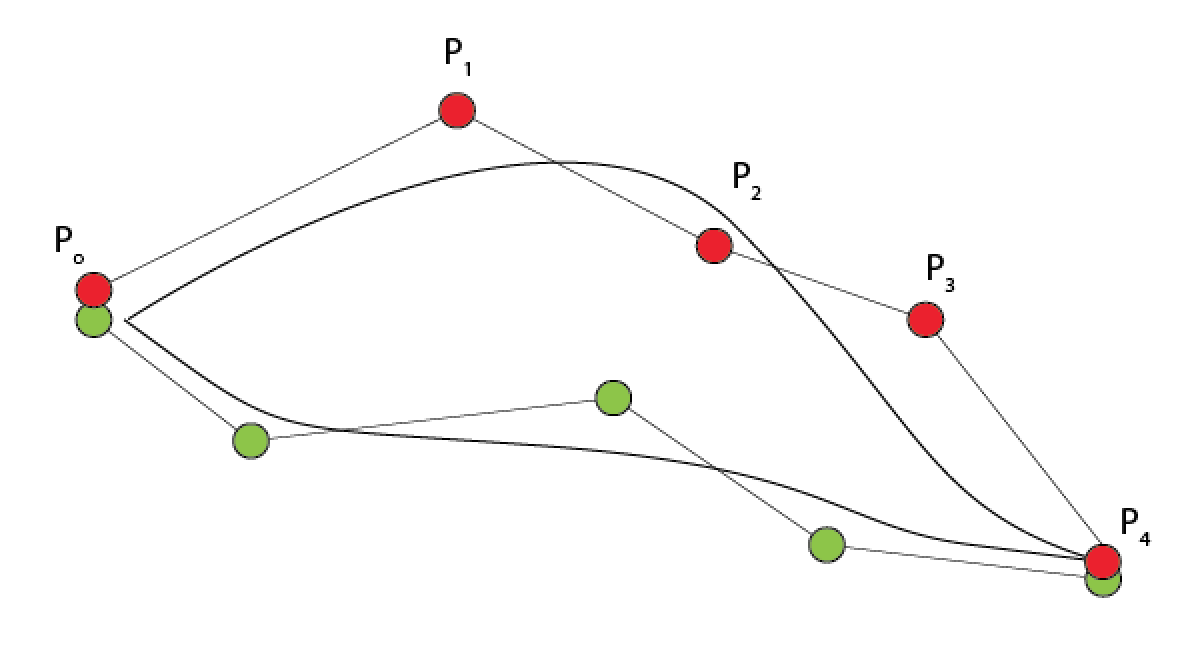
\includegraphics[width=06in]{twoCurves.png}
    \caption{Shows two quintic bezier curve with 5 control points}
\end{figure}

The curves are formed by computing the central points of the Ball with diameter $D$. The points on the curves are obtained by Linear Interpolation.

\subsection{Calculate the First Median Point on the Medial Curve}

Let $A_0$ be the start point of both curves $A$ and $B$ and  medial curve $C$. From the parametric equation given in \ref{eq:1} we found two points $A_1$ and $B_1$ on curves $A$ and $B$ respectively very close to start point $A_0$.
We first calculate the Angle Bisector Vector $BS$ by summing the vectors $A$ and $B$ and dividing by 2.

Now we need to compute the first median point $M_0$ on this Vector $BS$. That is given by the following equation,
\begin{equation}
  \label{eq:5}
M_0 = P(A_0,dis,BS)
\end{equation}

where $dis$ is the minimum value of $D/2$, magnitude($A1$) or magnitude($B1$).
Here,$D$ is the diameter of the fitting ball between input curves $A$ and $B$, such that it is tangential to both the curves.

\begin{figure} [t]
    \centering
    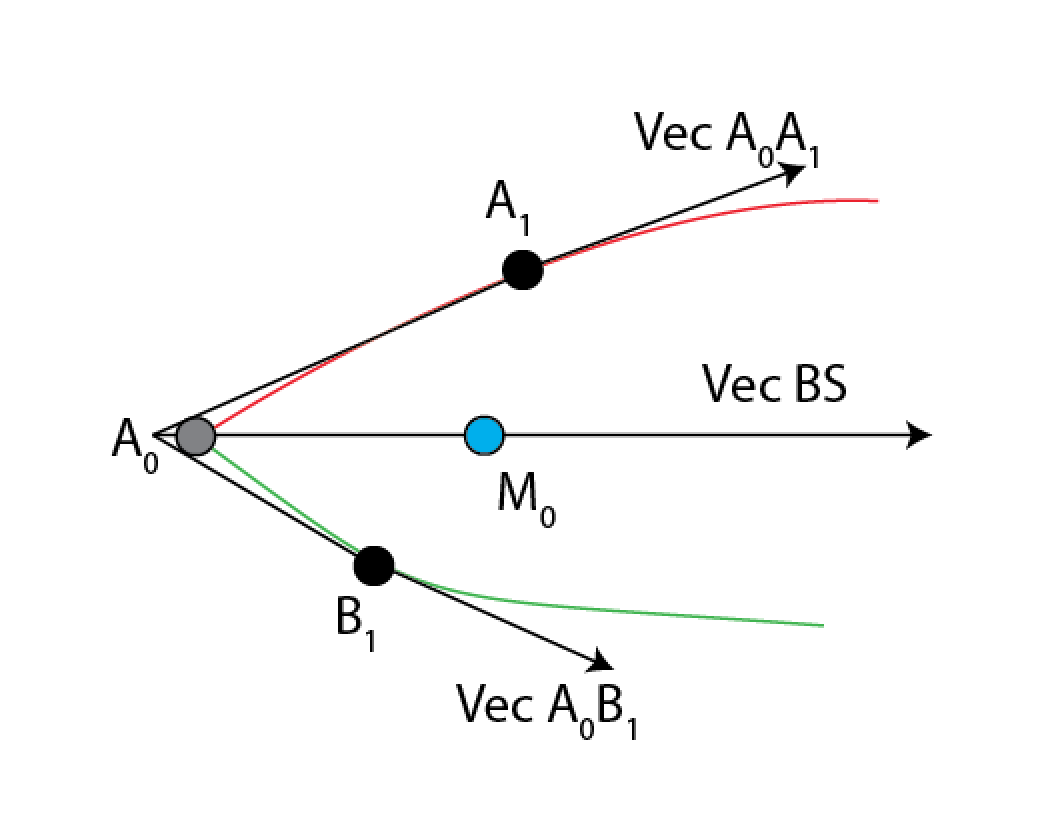
\includegraphics[width=05in]{bisector.png}
    \caption{Shows two quintic bezier curve with 5 control points}
\end{figure}

\subsection{Calculate the next median Point by guessing}

Calculate the tangent vectors $tanV_1$ and $tanV_2$ at points $A_1$ and $B_1$ respectively as below:

\begin{equation}
  \label{eq:3}
  \begin{aligned}
c_1 &= 4*(1-t)^3\\
c_2 &=12*(1-t)^2*t\\
c_3 &=12*(1-t)*t^2\\
c_4 &= t^3\\
Vector $ tanV_1$& = ($c_1$*v1+$c_2$*v2) + ($c_3$*v3 + $c_4$*v4)
\end{aligned}
\end{equation}
where, $v1, v2, v3$ $ and$ $ v4$ are the vectors between the respective control points $P_0, P_1, P_2, P_3, P_4$.

Here, $tanV_1$ is the calculated tangent vector. We can compute $tanV_2$, the respective tangent vectors at point $A_1$ and $B_1$ using aforementioned principles.

\begin{figure} [t]
    \centering
    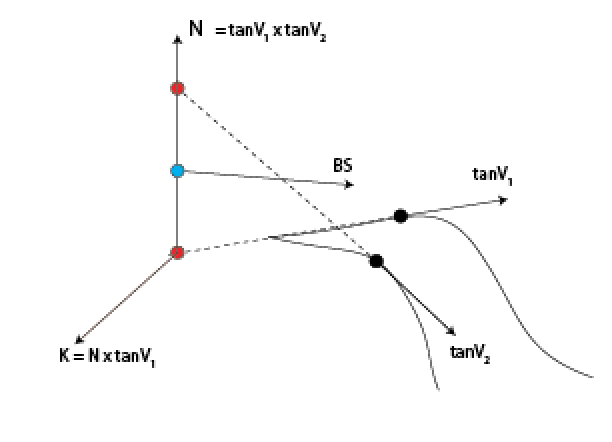
\includegraphics[width=06in]{intersection.png}
    \caption{Shows the two bisection point obtained by computing the normal Vector $N$}
\end{figure}
We compute the Bisection between the tangent vectors $tanV_1$ and $tanV_2$ and find two points on the bisector by the following calculation:

First, we get the normalized normal Vector $\underline{N}$:

\begin{equation}
  \label{eq:3}
  \begin{aligned}
    Vector $\underline{N}$ &= $tanV_1$ x $tanV_2$\\
Vector $\underline{NN}$ &= $N$/||$N$||
    
\end{aligned}
\end{equation}

We get the vector $A1B1$ between points $A_1$ and $B_1$. Also we compute the normalized perpendicular vector $K$ by taking cross product between $tanV_1$ and vector $N$. This allows to compute the point $P1$ as below:

\begin{equation}
  \label{eq:3}
  \begin{aligned}
float $ val$ &= dot($A_1B_1$,$ K$)/dot($tanV_1$,$K$)\\
Point $ P1$ &= P($B_1$,$val$,$ tanV_2$)
\end{aligned}
\end{equation}

We do the same to find the other point $P2$.

We add the points $P1$ and $P2$ to find the middle point $P3$. Also we add the normalized $tanV_1$ vector and normalized $tanV_2$ vector to get vector $V$. This helps us find $P4$ as below:

\begin{equation}
  \label{eq:3}
  \begin{aligned}
Point $ P4$ = P($P3$,$V$)
\end{aligned}
\end{equation}

Thus the final points we obtained from computing the bisection are $P3$ and $P4$. We use these points to compute the Vector $t$ between them and thus we get the guessed Median Point $MG_1$ as below:

\begin{equation}
  \label{eq:3}
  \begin{aligned}
Point $ MG_1$ = P($M_0$,$D/2,$t$)
\end{aligned}
\end{equation}

\begin{figure} [t]
    \centering
    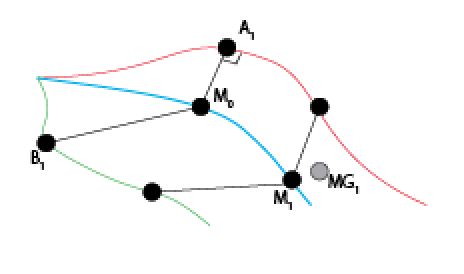
\includegraphics[width=04in]{parallelTransp.png}
    \caption{Shows the concept of parallel transport to find the next Median Point based on the current one}
\end{figure}

\subsection{Update the median point based on the Guess}

Even though we have the guessed median point, we know that its not precise. To compute the new median point from the guessed median point, we first find the projection of point $MG_1$ on curve $A$ and $B$ respectively.

%Finding the projection
To find the projection we shoot rays to each of the center point of the balls of the curve $A$ and find the ray with least distance $dis1$, to the point $MG_1$. 

Then if it is not the first point on the curve on the curve, then we check the projection side of the point $MG_1$ to the line between center balls points $c[id-1]$ and $c[id]$. We check to find if its on the line. If it is on the line , then we re compute the projection of point $MG_1$ on the $line(c[id-1],c[id])$ and compute the new distance $dis2$.

Similarly if it is not the last point on the curve, then we check the projection side of the point $MG_1$ to the line between center balls points $c[id]$ and $c[id+1]$. We check to find if its on the line. If it is on the line , then we re compute the projection of point $MG_1$ on the $line(c[id],c[id+1])$ and compute the new distance $dis3$.

We compare the three distances $dis1, dis2 & dis3$ and get the projected point $PA_1$ which has the least value.We do the same process for curve $B$ and find the projected point $PB_1$.

Likewise, we also calculate the tangent vectors $tanPA_1$ and $tanPB_1$ at points $PA_1$ and $PB_1$ respectively. At this point with the help of these two points and tangent vectors, we call the bisection method as explained above to compute the two bisected points $BB1$ and $BB2$.

We create a line between $BB1$ and $BB2$ and find the projection of $MG_1$ on this line which is basically the updated median point as below:

\begin{equation}
  \label{eq:3}
  \begin{aligned}
Point $ M_1$ = project($MG_1$,$BB1$,$BB2$)
\end{aligned}
\end{equation}



\subsection{Calculate the Median Line}
Computing the median lines needs computation of all the median points. We can get the First Median Point and the next Median Point as aforementioned. We iterate the computation part of guessing the next median and updating the same point with precision by feeding last computed median point as the first median point at each iteration. We keep a check such that the distance between the last median point and the end center point of the curve should be lesser than $D/2$.

\begin{equation}
  \label{eq:3}
  \begin{aligned}
while ( n(V(last.M, A.C[A.n-1])) > D/2 && i < 70){\\
Point $ p$ = guessNextMedian()\\
Point $ pnew$ = updateMedianPoint()\\
}
\end{aligned}
\end{equation}


\begin{figure} [t]
    \centering
    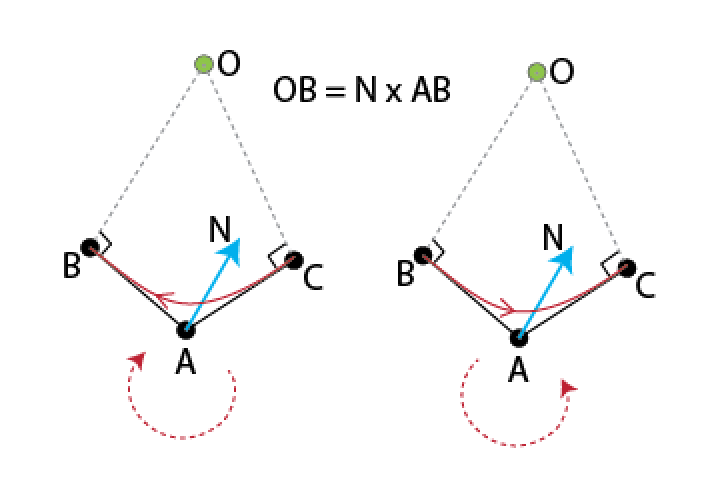
\includegraphics[width=04in]{arcCenter.png}
    \caption{Shows the strategy implemented to computed the Arc Center $O$}
    \label{fig:arcCenter}
\end{figure}
\subsection{Computing the transverse Arcs at each Median Point}
At this point, we have stored each of the median points location, $M_0, M_1, M_2, M_3 ...$. Also, each of the median points have access to the nearest projection points on the curves $A$ and $B$. For example, median point $M_0$ has point $A_1$ & $B_1$ on curve $A$ and $B$ respectively.

Lets consider any three set of such points namely $A$, $B$ and $C$ as shown in Figure ~\ref{fig:arcCenter}.With these three points we compute the Arc Center point $O$. We get vector $OB$ and vector $OC$ and compute the angle $a$ between them.To understand if $O$, $B$, and $C$ are clockwise or anticlockwise we check if $ det(OB,OC)$ is negative or positive respectively.If it is clockwise, we first compute the vector $I$ and $J$ as below:
\begin{equation}
  \label{eq:3}
  \begin{aligned}
$ vec I &= normalized(OB)$\\
$ vec J &= normalized((OC x OB) x OC))$

\end{aligned}
\end{equation}

Then we compute the points on the arc by the following equations:
\begin{equation}
  \label{eq:3}
  \begin{aligned}
$ vec VN &= vec (r*(i/n), V(O,pn))$\\
$Point OA_1 &= P(O,VN)
\end{aligned}
\end{equation}

where, $OA_1$ is one of the computed points on the arc,
Point $pn$ is the rotated point around $O$ in the plane of vectors $I$ and $J$ 
\section{Parallel Transport and Worm}
\begin{figure} [t]
    \centering
    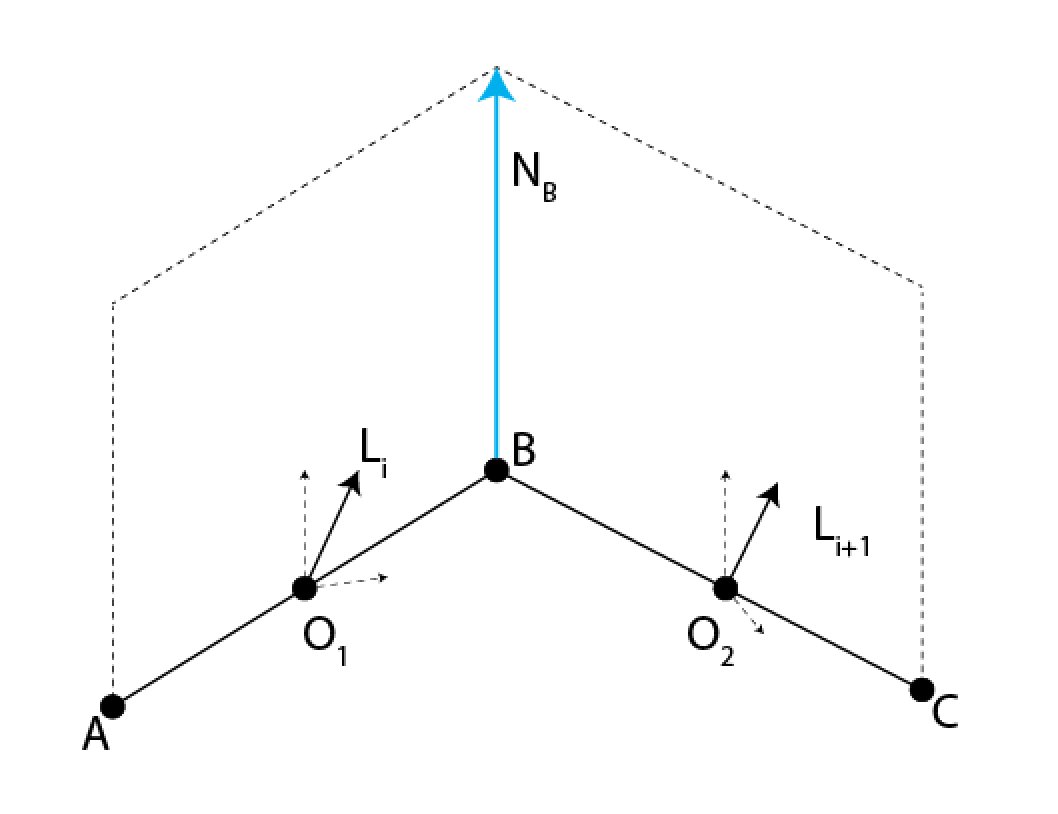
\includegraphics[width=04in]{parallelTransp2.png}
    \caption{Shows the concept of parallel transport to find the correct normal direction for the next center ball point on the median curve}
    \label{fig:parTransp2}
\end{figure}
\subsection{Median Rope by Parallel Transport}
We use the concept of parallel transport to make circles at each median point on the median curve. Parallel transport helps us to keep the normal vector direction aligned with each other for all the median points. Lets say we have three consecutive median control points $A$, $B$ and $C$ as shown in Figure ~\ref{fig:parTransp2}. Let $O_1$ and $O_2$ be two points on the median curve , wherein our aim is to keep the Normal vector direction of $L_i$ same as Normal vector direction at point $O_2$, which is given by $L_i_+_1$. We computed the vector $N_B$ by taking the cross product of vectors $AB$ and $BC$. The we decompose the vector $L_i$ in the direction of $N_B$ and another component in another direction by the following equation:

\begin{equation}
  \label{eq:3}
  \begin{aligned}
$L_i$ = $x$*$N_B$ + $y$*$(AB$ x $N_B)$
\end{aligned}
\end{equation}

where $x$ and $y$ are some unknown constants. 

Similarly, we computed the vector $L_i_+_1$ as shown below:
\begin{equation}
  \label{eq:3}
  \begin{aligned}
$L_i_+_1$ = $x$*$N_B$ + $y$*$(BC$ x $N_B)$
\end{aligned}
\end{equation}

We solve the above two equations to find the direction of the vector $L_i_+_1$. We do the same to all the median points to find the normal and the oriented circles. At the next step we form the quads around these circles to form the rope.


\subsection{Making of the Worm}
We begin by forming a vector $C_1C_2$ from from first center of ball to the next one on the median curve. We get the cross product of this vector with the vector from the current center of ball to the projected point on Curve $B$. We call the second vector $BB$. This cross product gives the vector $PP$ which is perpendicular to both$C_1C_2$ and $BB$. We again take the cross product of vector $PP$ with the vector $C_1C_2$ to find a vector $VF$ pointing in the plane of the vectors $C_1C_2$ and vector $BB$.

We get the number of subdivision of quads, $sd$ from the user and make two dimensional $float$ variables $'c'$ and $'s'$ to store the value of $r*cos(2*PI*m/sd)$ and $r*sin(2*PI*m/sd)$, where $r$ is given by the average sum of distance to the projected point on Curve $A$ and $B$ for both the current center ball point and the previous one. We use these values to compute the two perpendicular directors of the center points $C_1$ and $C_2$, given by the following equation:
\begin{equation}
  \label{eq:3}
  \begin{aligned}
$ Point PT = Point (p1,c,VF,s, (VF x C_1C_2))$
\end{aligned}
\end{equation}

where, $p1$ is the summation of points $C_1$ and $C_2$.

This was the computation of Point $PT$ for 1st two center ball points on the median curve.

Next we iterate over the rest of the center ball points on the median curve. We compute vector $I$ and $IP$ which are respectively vector between previous center point  and current center point and vector between current center point and next one.Further we compute vector $IPM$ by subtracting vector $I$ from vector $IP$.We also get the normal vector $N$ for vector $I$ and vector $IP$.

We compute set of points $PT[][]$ similar to point $PT$ computed as shown before by the following equation:

\begin{equation}
  \label{eq:3}
  \begin{aligned}
$ Point PT[][] = Point ((C_i+C_i_+_1),c,I,s,J)$
\end{aligned}
\end{equation}

We use these set of points to form the shape for the worm, which is essentially a series of circular quads having radius $r$ such that both curves $A$ and $B$ are tangential to it.


\section{Implementation details and some cautions}

\subsection{Class Nearest}
This Class in rope.pde contains the data structure to store the closest projection in a rope to a certain point. It stores, the projection point, projection distance, the id of the projected point and whether the point is in the middle of an edge.

\subsection{Class Median}
This Class in rope.pde creates the data structure to save the median point $P$ with two other Nearest Objects, storing the respective nearest points on each Curve $A$ and $B$. 

All the medians are stored in an arraylist $mps$

\subsection{Class Rope}
The given class rope is used to make a new $MPS$ object which is the median curve. we implement the computation of curve points in the function $calRope()$ under rope.pde.Likewise we implemented $calTangent()$ to compute the tangent vectors at any point on the curve.

The projection of any point on the curve is implemented in $calProject()$ function which returns a Nearest object. It takes the id of the point on the curve and the external point to be projected as input.

\subsection{Median Point Implementation}
The function $calfirstMedian()$ computes the first median point by taking three points as input.

The function $guessNextMedian()$ returns the next best guessed median point on the median curve by taking the last computed median point as an input

The function $updateMedianPoint()$ returns the precise next median point on the median curve by taking the guessed median point as input along with the id's of the last projected points on the left and right curve.


\subsection{Median Curve Implementation}

The function $calMedian()$ iterates to compute the first median point, guessed median point and updated median point repeatedly, till the length of the median curve cannot fit any new median point to make the curve.

\subsection{Parallel Transport & Worm Implementation}

The function $showQuad()$ under Ropes.pde implements the parallel transport. Both full worm and half worm structure is implemented by the $showWorm()$ function to be found in Ropes.pde.

\subsection{Control methods}
We can control the output as below \begin{enumerate}
 \item mouse + key 'R or r' = vibrate the output
 \item mouse + key 'X or x' = rotate X axis
 \item mouse + key 'Y or y' = rotate Y axis
\item key 'A' = show animation of the morph
\item key 'C or c' = show the arcs
\item key 'D or d' = show the net ( arcs and curves)
\item key 'F or f' = show the worm
\item key 'G or g' = show the half worm

 \end{enumerate}
 
 
 
\section{Program Output}

\begin{figure} [H]
    \centering
    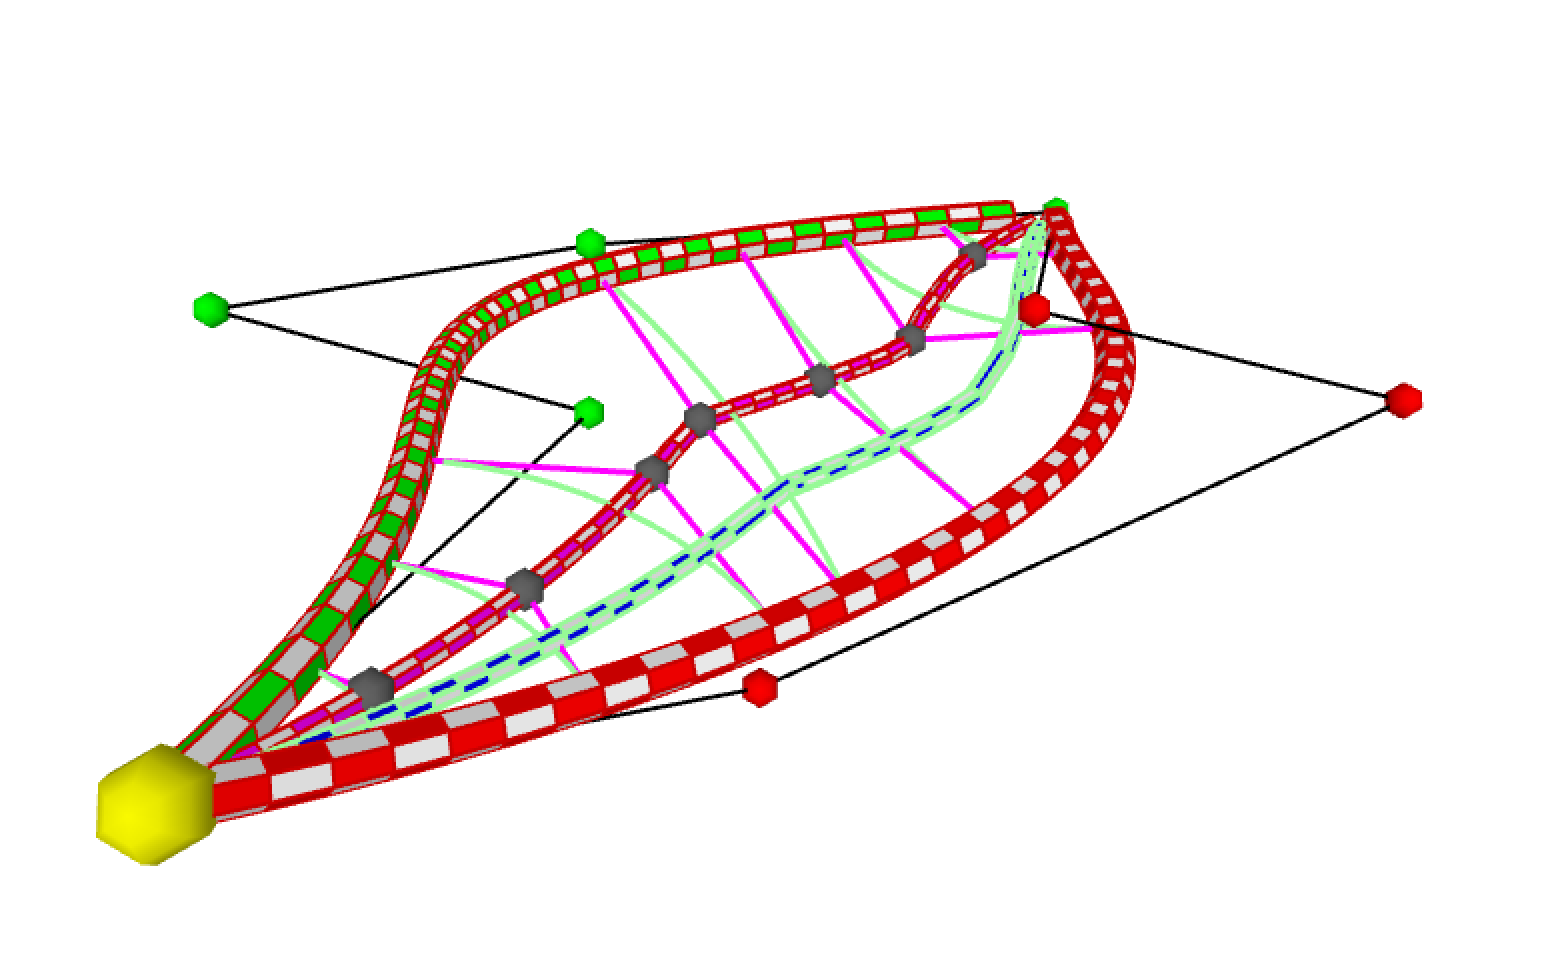
\includegraphics[width=04in]{ssAnim.png}
    \caption{Screenshot of the animating morph via the median curve from Curve A to B}
\end{figure}



\begin{figure} [H]
    \centering
    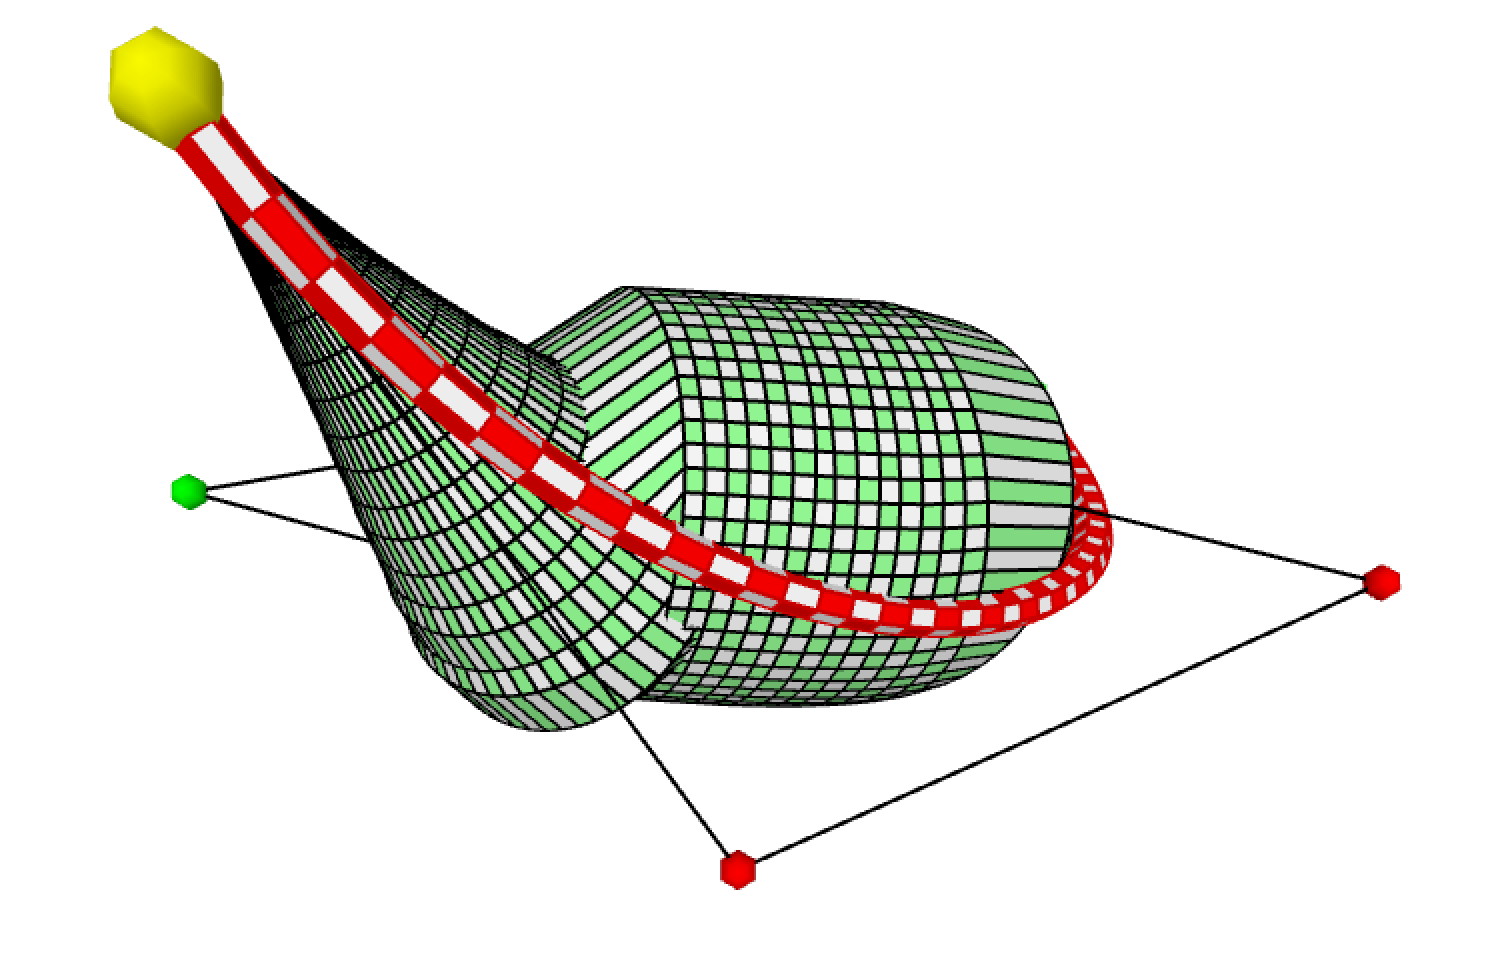
\includegraphics[width=04in]{wormFull.png}
    \caption{Screenshot of the worm structure between the two tangential rope}
\end{figure}

\begin{figure} [H]
    \centering
    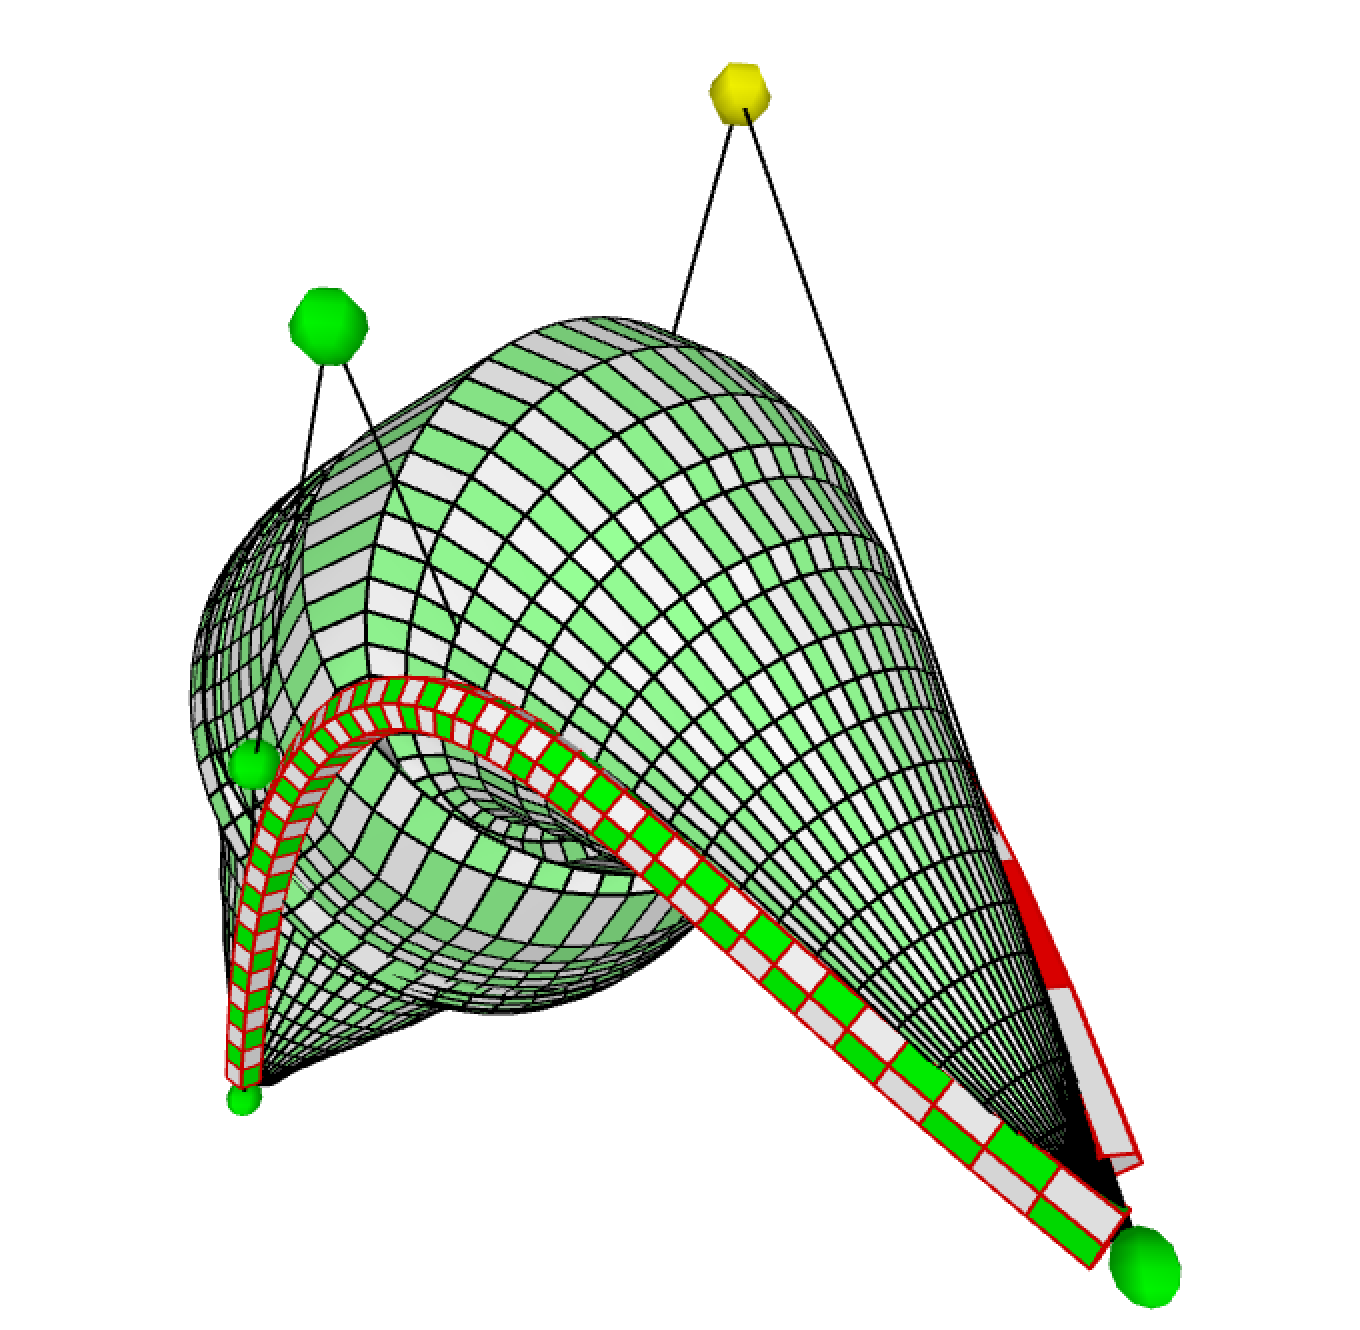
\includegraphics[width=04in]{wormFull2.png}
    \caption{Screenshot of the worm structure between the two tangential rope}
\end{figure}


\begin{figure} [H]
    \centering
    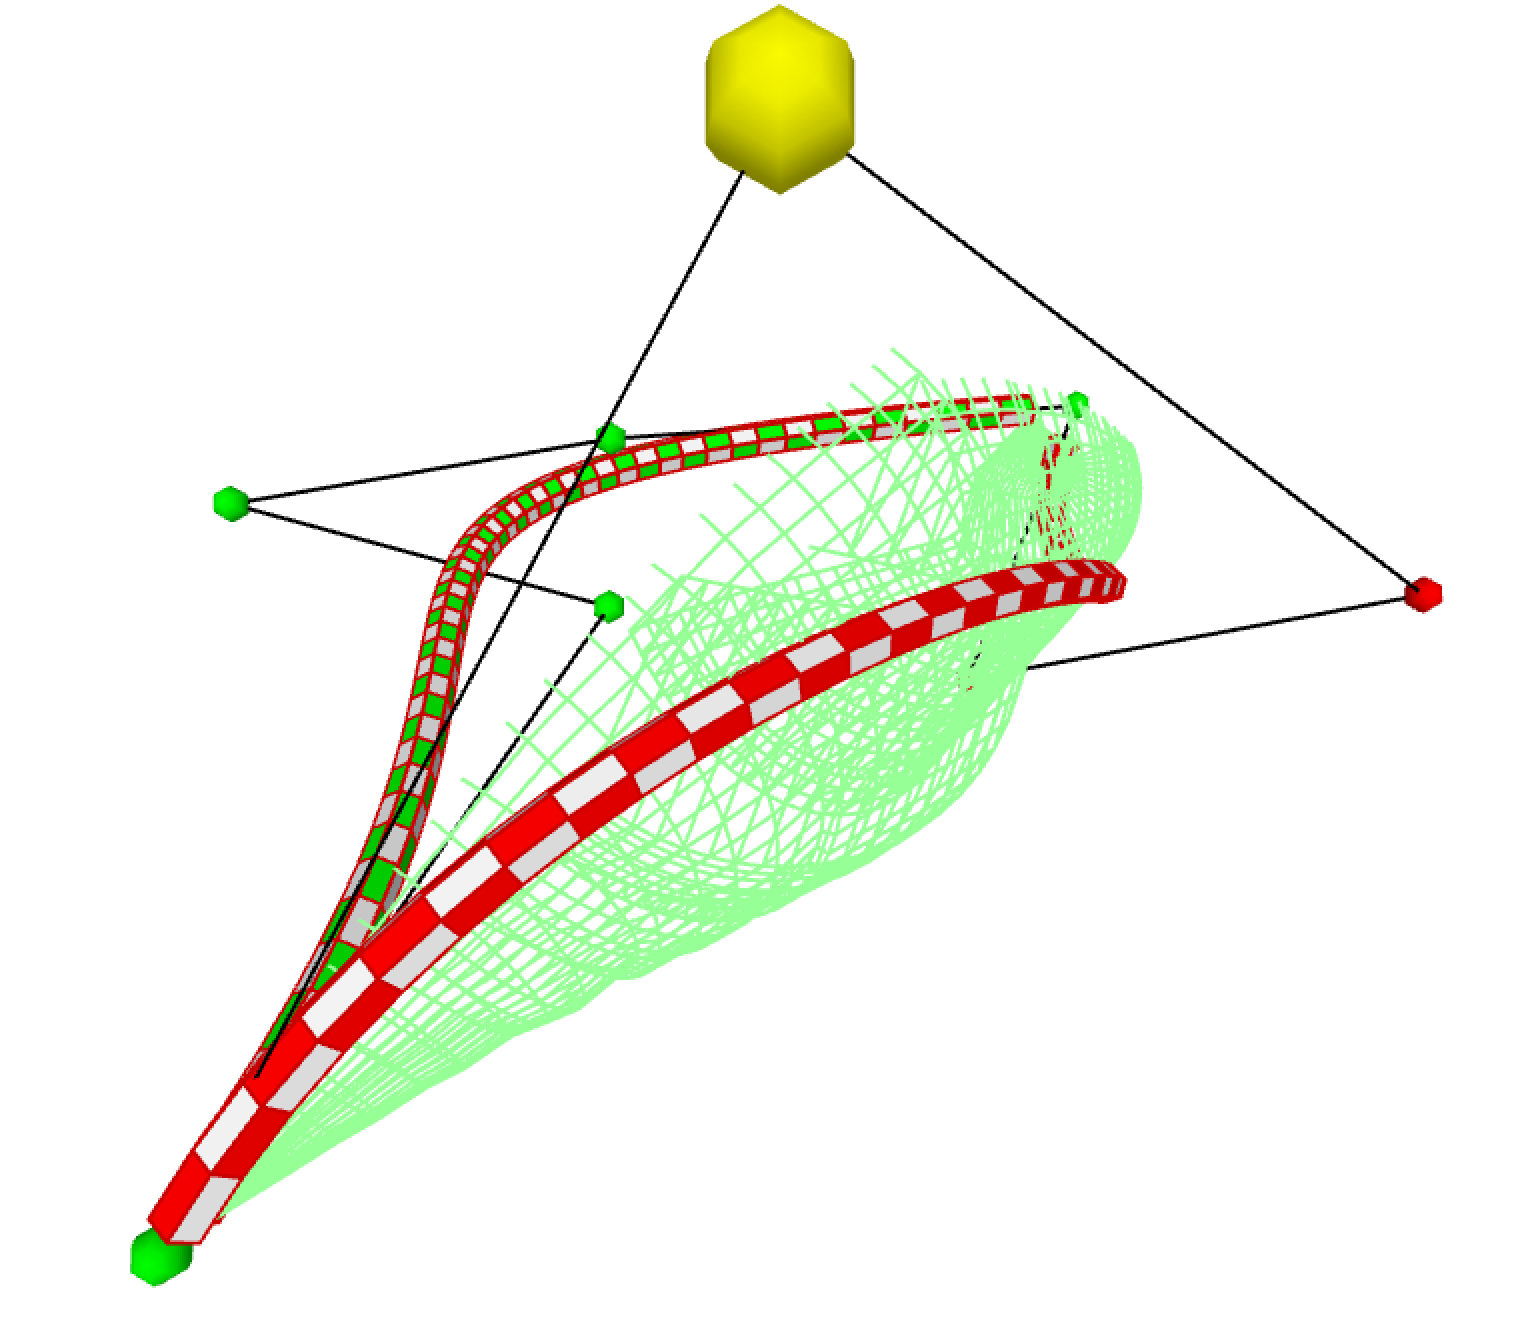
\includegraphics[width=04in]{wormHalf.png}
    \caption{Screenshot of the half worm structure between the two tangential rope}
\end{figure}

\begin{figure} [H]
    \centering
    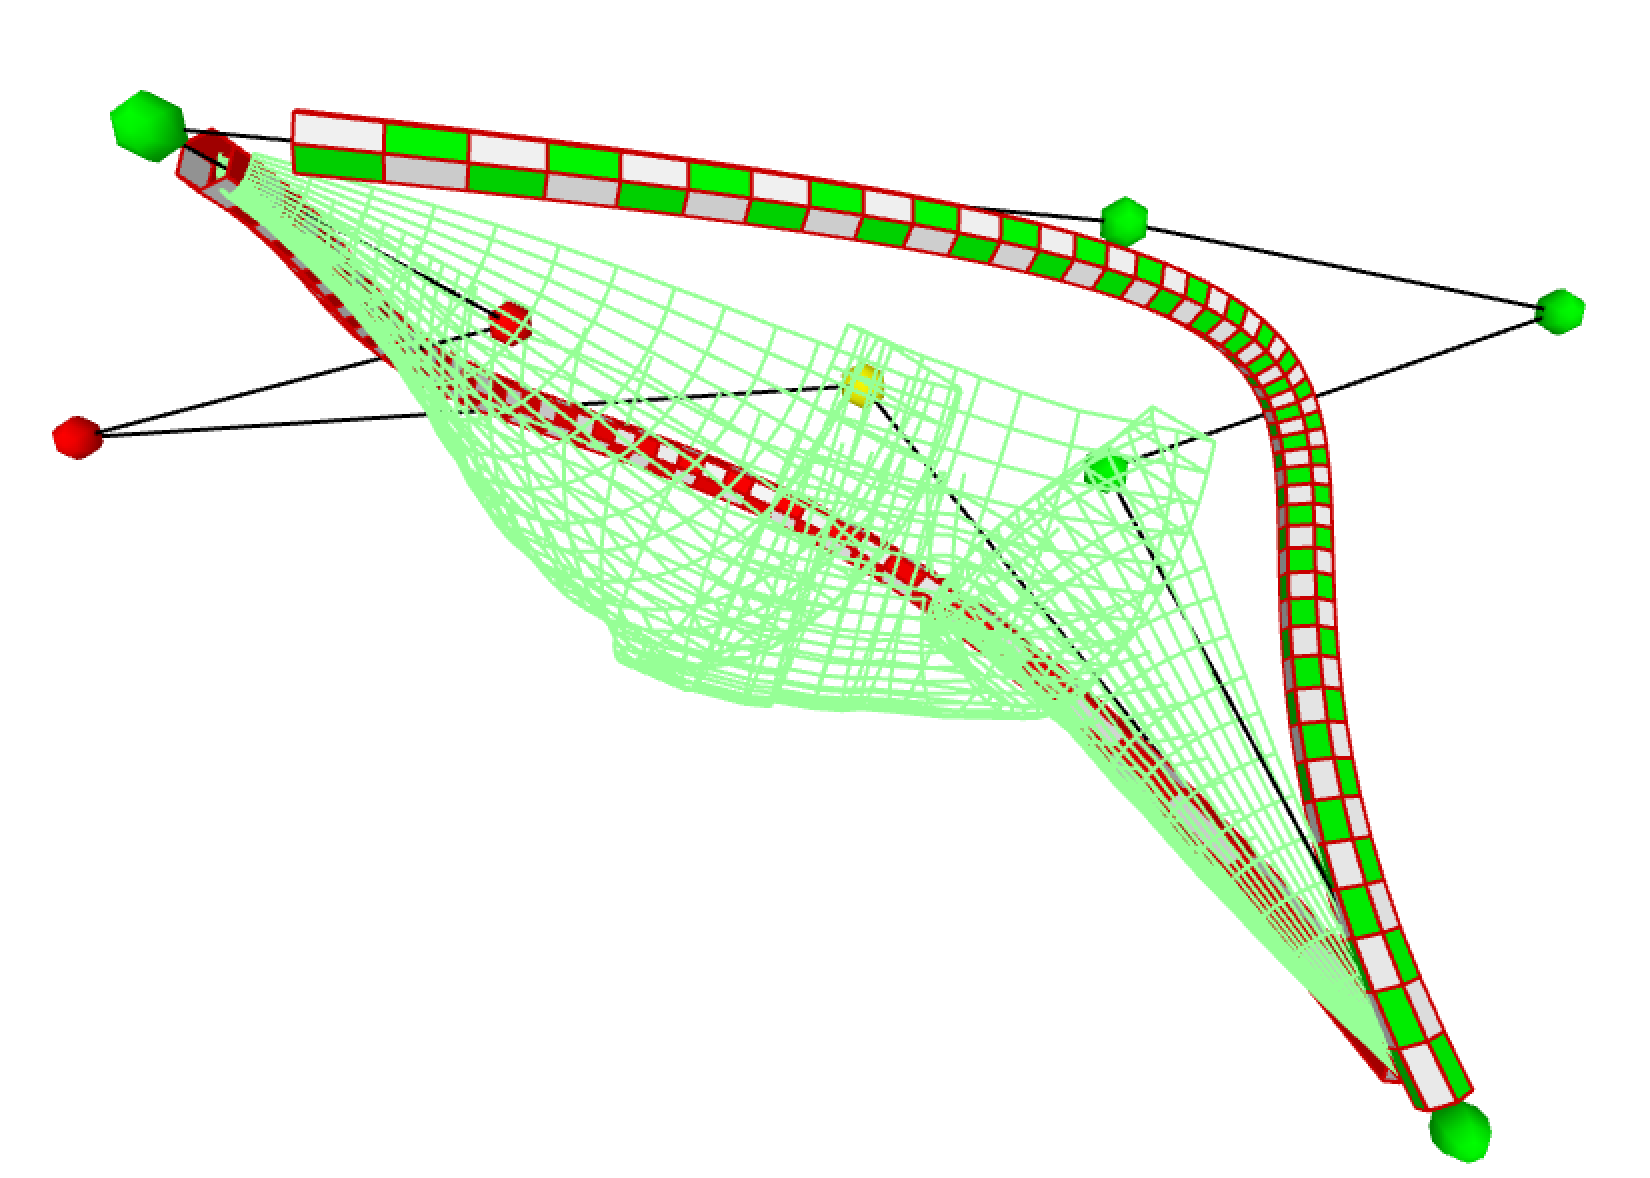
\includegraphics[width=04in]{wormHalf2.png}
    \caption{Screenshot of the half worm structure between the two tangential rope}
\end{figure}





\section{Problems and Loose Ends}

Though our implementation gives good result for the most part and successfully outputs the intended worm and half worm structure along with the computation of the median curve, it does have its own set of cracks and loose ends. While playing with the input curves and manipulating in complex ways we figured that at times if the third or fourth control point of one of the input curves is stretched a bit far away from the other input curve, the computed median curve extends beyond the end point and gives erroneous output.

\begin{figure} [H]
    \centering
    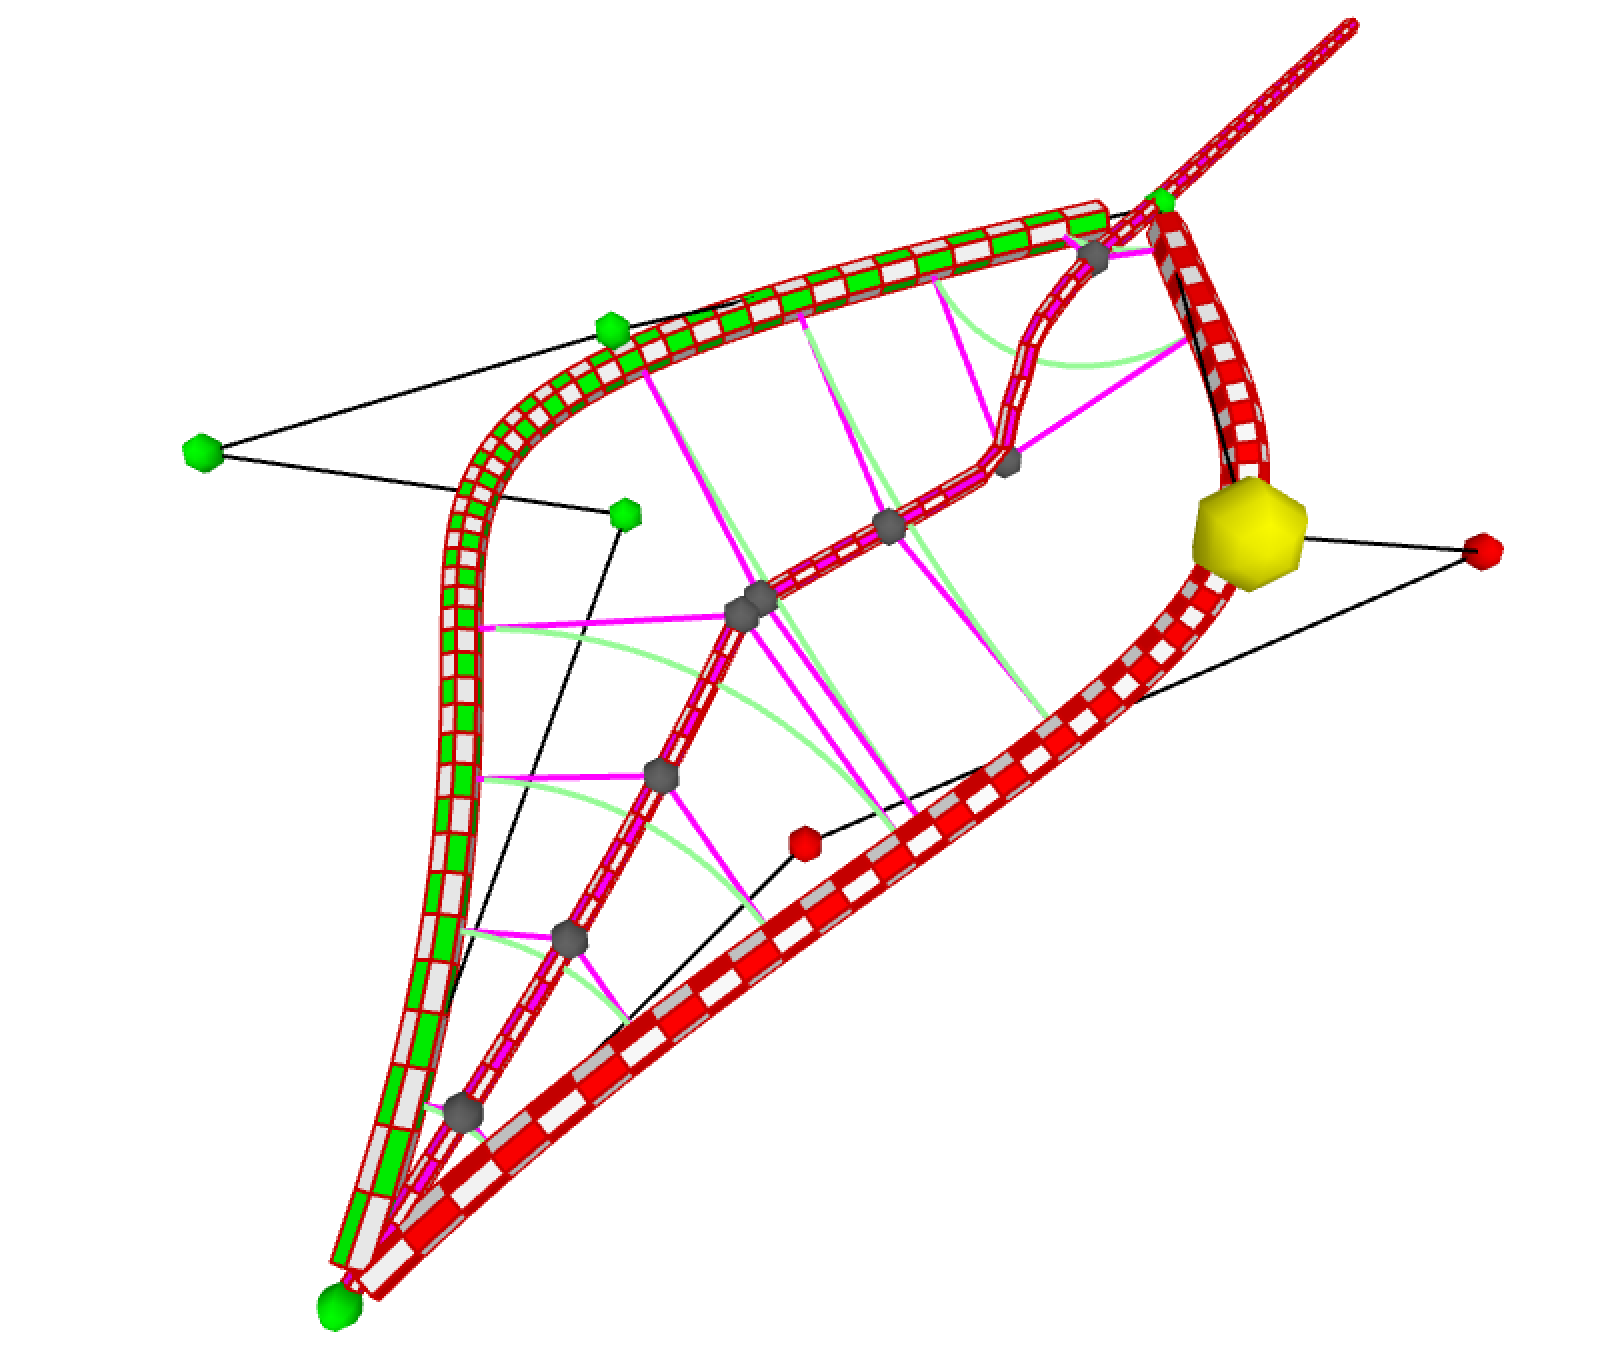
\includegraphics[width=04in]{problemCase1.png}
    \caption{Screenshot of the median curve extends itself outward on one of the ends, if the control points are stretched too far upwards.}
\end{figure}

\begin{figure} [H]
    \centering
    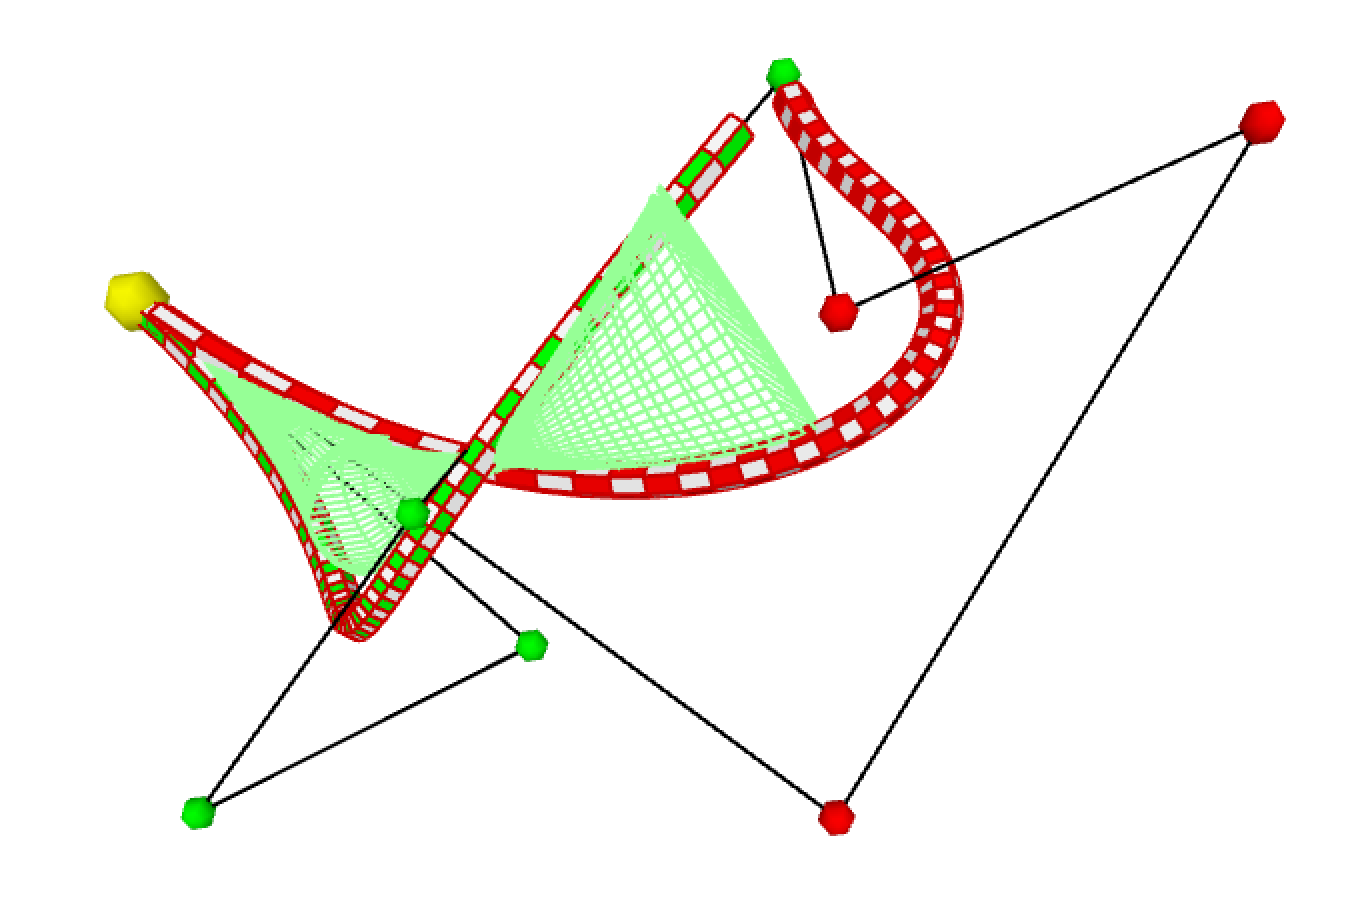
\includegraphics[width=04in]{problemCase2.png}
    \caption{Screenshot of one of the cases for half worm when the two input curves entangle against each other and the half worm ends up not forming itself}
    \label{fig:halfWorm2}
\end{figure}

Another similar problem was observed in the graphical representation of the halfworm structure. When the input curves are manipulated such that they overlap each other and entangle, the half worm structure ends up forming only on one half of the area as shown in Figure ~\ref{fig:halfWorm2}





\section{Conclusion, discussion and reliability}
\end{document}
